\documentclass[tikz,border=5pt]{standalone}
\usepackage{amssymb,amsmath}
\newcommand{\C}{\mathbb{C}}
\newcommand{\CP}{\mathbb{CP}}
\newcommand{\Res}{\operatorname{Res}}
\begin{document}
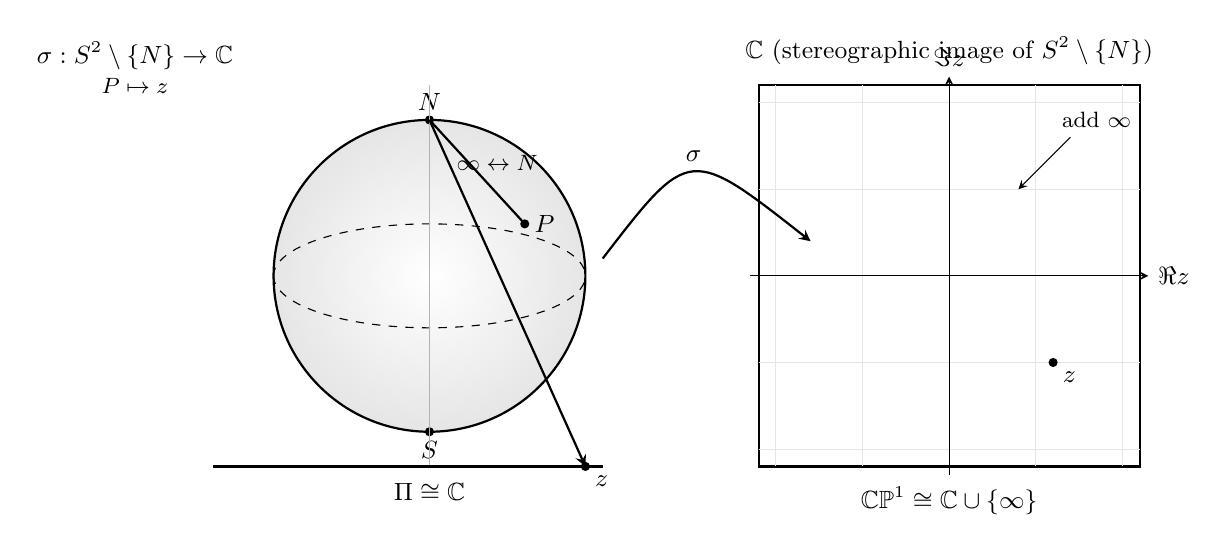
\begin{tikzpicture}[font=\small,>=stealth,scale=1.1]
	
	%------------------------------
	% Sphere S^2
	%------------------------------
	\begin{scope}[shift={(-3,0)}]
		% Outer circle (equator projection)
		\shade[inner color=white, outer color=gray!20, draw=black, thick]
		(0,0) circle (1.8);
		
		% "Equator" ellipse
		\draw[dashed] (-1.8,0) arc (180:360:1.8 and 0.6);
		\draw[dashed] (-1.8,0) arc (180:0:1.8 and 0.6);
		
		% North pole N
		\coordinate (N) at (0,1.8);
		\fill (N) circle (1.5pt) node[above] {$N$};
		
		% South pole S
		\coordinate (S) at (0,-1.8);
		\fill (S) circle (1.5pt) node[below] {$S$};
		
		% A point P on the sphere (somewhere on front-right)
		\coordinate (P) at (1.1,0.6);
		\fill (P) circle (1.5pt) node[right] {$P$};
		
		% Vertical line through S (projection of the axis)
		\draw[gray!60] (0,-2.2) -- (0,2.2);
		
		% Plane z=0 (equatorial plane)
		\draw[thick] (-2.5,-2.2) -- (2.0,-2.2);
		\node at (0,-2.5) {$\Pi \cong \C$};
		
		% Intersection of line N--P with plane Pi
		% Choose some point Q for intersection
		\coordinate (Q) at (1.8,-2.2);
		\fill (Q) circle (1.5pt) node[below right] {$z$};
		
		% Line from N through P to Q (stereographic projection line)
		\draw[thick,->] (N) -- (Q);
		\draw[thick] (N) -- (P);
		
		% Arrow indicating stereographic projection map
		\node[align=center] at (-3.4,2.4)
		{$\sigma:S^2\setminus\{N\}\to\C$\\ \footnotesize $P\mapsto z$};
		
		% Mark infinity at N
		\node[right] at (0.2,1.3) {\footnotesize $\infty \leftrightarrow N$};
	\end{scope}
	
	%------------------------------
	% Complex plane as CP^1 minus infinity
	%------------------------------
	\begin{scope}[shift={(3,0)}]
		% Rectangle for C
		\draw[thick] (-2.2,-2.2) rectangle (2.2,2.2);
		\node at (0,2.6) {$\C$ (stereographic image of $S^2\setminus\{N\}$)};
		
		% Grid (light)
		\foreach \x in {-2,-1,...,2}
		\draw[gray!20] (\x,-2.2) -- (\x,2.2);
		\foreach \y in {-2,-1,...,2}
		\draw[gray!20] (-2.2,\y) -- (2.2,\y);
		
		% Axes
		\draw[->] (-2.3,0) -- (2.3,0) node[right] {$\Re z$};
		\draw[->] (0,-2.3) -- (0,2.3) node[above] {$\Im z$};
		
		% Point z
		\fill (1.2,-1.0) circle (1.5pt) node[below right] {$z$};
		
		% Indicate infinity as "added point"
		\node at (1.7,1.8) {\footnotesize add $\infty$};
		\draw[->] (1.4,1.6) -- (0.8,1.0);
		
		% Label for CP^1
		\node at (0,-2.6) {$\CP^1 \cong \C\cup\{\infty\}$};
	\end{scope}
	
	% Arrow S^2 -> C: stereographic projection
	\draw[->,thick]
	(-1.0,0.2) .. controls (0.0,1.5) .. (1.4,0.4)
	node[midway,above] {$\sigma$};
	
\end{tikzpicture}
\end{document}
